\section{Methods}
\label{sec:Methods}

Although Section \ref{subsec:Objectives} clearly specified our objectives, it did so on a very high level, giving us the freedom to choose the techniques and methods we employed to achieve them. These decisions were primarily influenced by the background research found in Chapter \ref{sec:Background} and could be split into two distinct but interconnected parts.

\subsection{Structural Embeddings Creation}

In order to construct our protein structure embeddings we decided to create a neural network that would be trained on a specific classification task, making use of protein 3D structures, involving as many proteins as possible in order to maximise the number of created embeddings. Once the model was trained we would then extract the protein structural embeddings from one of the model layers and use them in our DTIs models. This is commonly known as transfer learning where we use the data or knowledge gathered by solving one task to solve a different but closely related one \citep{Zhuang2019}. Figure \ref{fig:Embeddings_Methodology} summarises our methodology.

\subsubsection{Dataset}

Given that each protein has one or more molecular functions we decided that it would be the perfect classification task to build our embedding model around. 

We started by using all the predicted human proteins from the AlphaFold protein structure database \citep{Jumper2021, Varadi2022} and retrieving all the protein accession numbers and sequences. Then using these protein accession numbers we extracted each protein's molecular functions from UniProt \citep{UniProt_Paper}. To simplify the problem we decided to only focus on the most prevalent molecular function among our proteins, which was "DNA Binding", turning the problem from multi-label to single.

For each protein we used Protr \citep{ProtR_Paper}, mentioned in Subsection \ref{subsec:Protein_Sequence_Descriptors}, to retrieve its protein sequence descriptors and PSSM, UniProt \citep{UniProt_Paper} for its protein sequence embedding and amino acids embedding, \citet{Peptides} and more specifically its aaDescriptors function to calculate 66 amino acid descriptors and finally its contact map using a threshold of 10\AA {} using the nanoHUB library, created precisely for this type of task \citep{nanoHUB_Library}.

The amino acid descriptors and embeddings, PSSM, and contact maps were all saved as NumPy files in order to easily pass them on to the neural network during its training.

We then performed data cleaning, removing any proteins with missing descriptors and any proteins whose acid descriptors and embeddings, PSSM and contact maps were mismatched, meaning having a different amount of amino acids. This process decreased the size of available proteins from 11,202 to 11,034, with 1,989 classified as having a positive "DNA Binding" and 9,045 as having a negative "DNA Binding".

\subsubsection{Holdout Test Sets}

Given that this dataset and the subsequent embedding model were just a means to an end to create as many embeddings as possible we decided against using a holdout test set as the performance of the embedding model was not of interest to us.

\subsubsection{Feature Selection}

To improve our models' predictive performance and reduce their training time we used the recursive feature elimination with cross-validation function (RFECV) offered by Scikit-Learn \citep{scikit-learn} using a random forest classifier and 5-fold cross-validation.

Before running RFECV we decided to reduce the number of tripeptide protein sequence descriptors using principal component analysis (PCA), a dimensionality reduction method, to reduce their size to a number holding 95\% of their variance. As a result, PCA managed to reduce their number from 8000 to 4813 and RFECV was then able to reduce the amount of features from 7757 to 144.

\subsubsection{Embeddings Creation Process}

Inspired by the study conducted by \citet{Jiang2020} we decided to use a very similar architecture, showcased in Figure \ref{fig:Embeddings_NN_Architecture}.

Our architecture utilised a protein graph, using a sparse contact map, with a threshold of 10\AA {}, as its adjacency matrix and amino acid descriptors, embeddings and PSSM as its node features, fed into three PyTorch Geometric graph convolutional layers, with ReLU activation and a global mean pooling layer at the end. The protein graph representation would then be flattened using two linear layers and concatenated with the protein sequence descriptors representation which would have passed through three linear layers, again using ReLU activation but also dropout layers. Once concatenated they would be passed through two more linear layers, again with ReLU activation and dropout layers, and a prediction would be made regarding the "DNA Binding" molecular function.

The neural network was trained using balanced batches of 16 over 50 epochs, which we found were enough for our model to converge. Our model was optimised using Adam with a learning rate of 0.00001 and weight decay of 0.001 and for our loss function we used binary cross entropy loss.

Once the model was trained we used a forward hook on the second dense linear layer before the concatenation, showcased in Figure \ref{fig:Embeddings_NN_Architecture}, and performed a sequential forward pass over all of our proteins. Each forward pass would extract the embedding with 256 dimensions and place it into a dictionary which once complete was pickled for easy storage and retrieval.

\begin{figure}[!h]
    \centering
    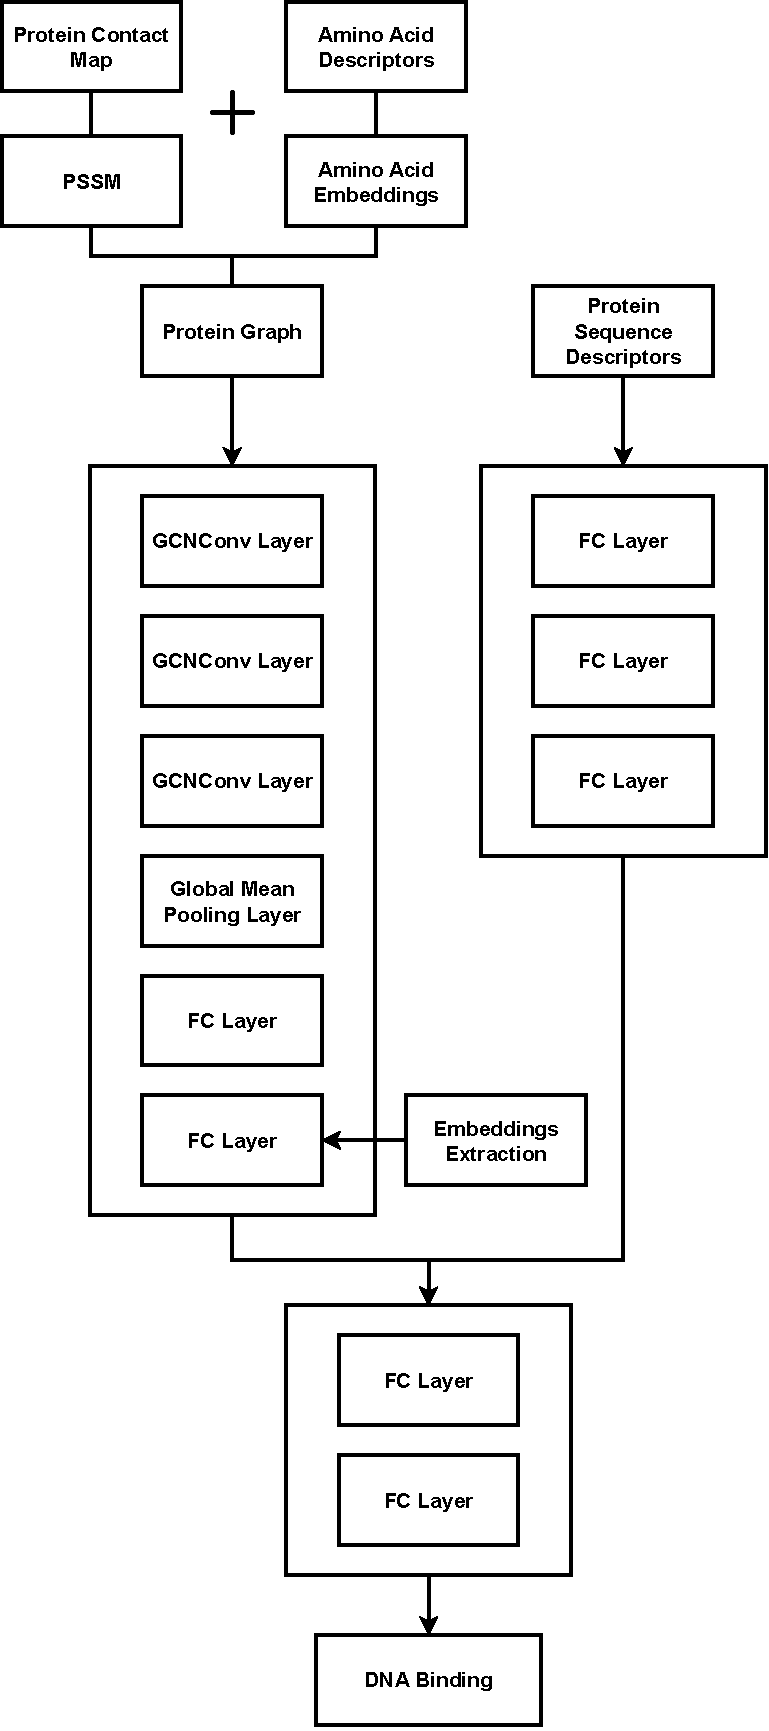
\includegraphics[width=0.95\linewidth]{images/Embeddings_NN_Architecture.pdf}    
    \caption{Figure showcasing our embedding model's architecture.}
    \label{fig:Embeddings_NN_Architecture} 
\end{figure}

\begin{figure*}[!h]
    \centering
    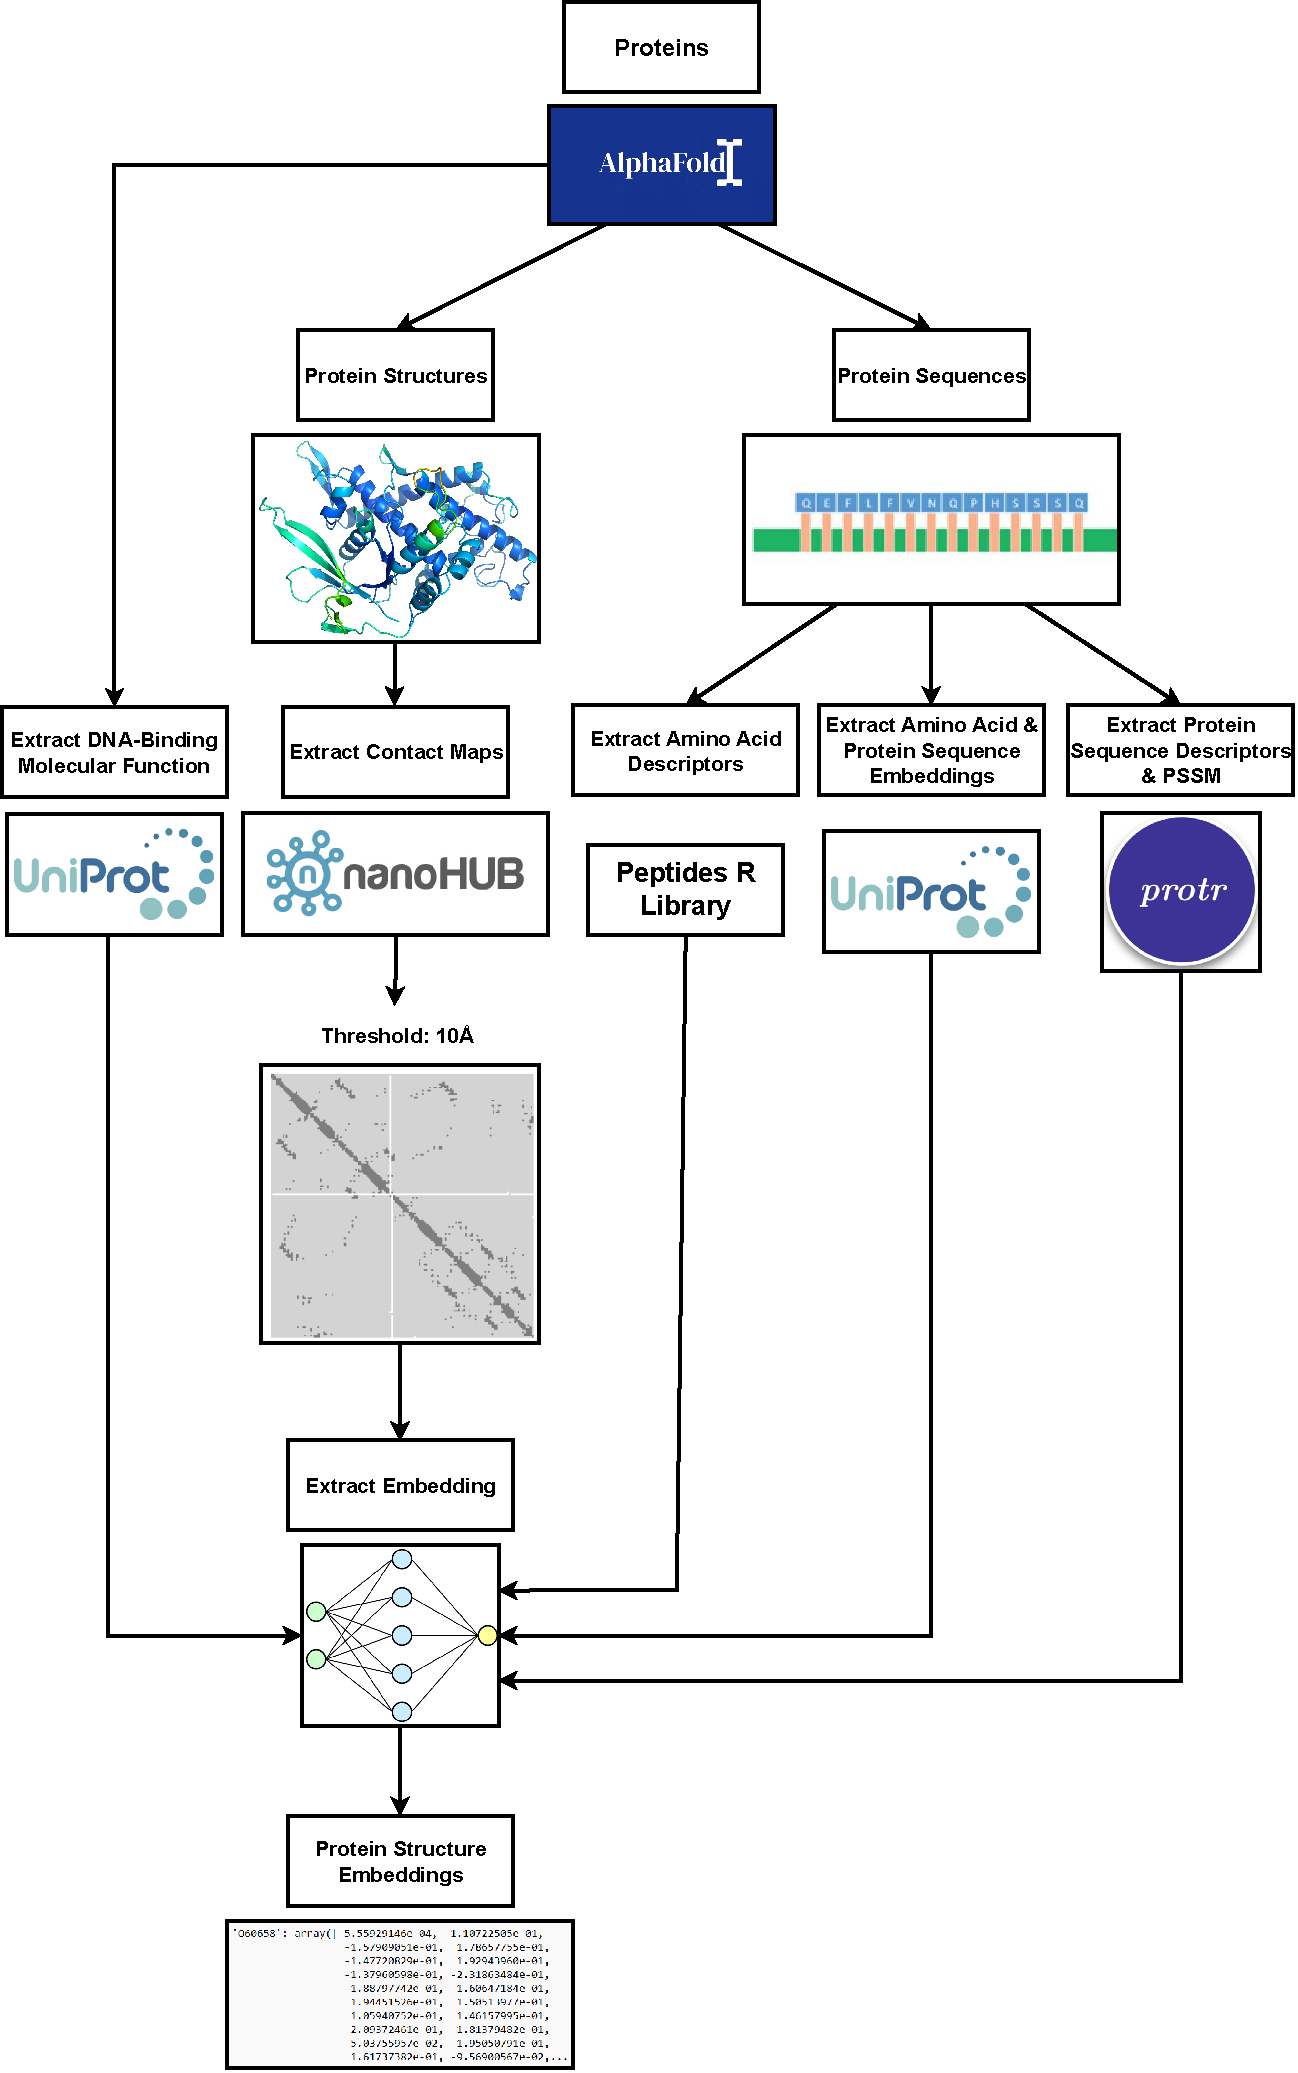
\includegraphics[width=0.78\linewidth]{images/Embeddings_Methodology.pdf}    
    \caption{Figure showcasing our methodology behind the embedding model.}
    \label{fig:Embeddings_Methodology} 
\end{figure*}

\subsection{Drug-Target Interactions Models}

To simplify the problem we had first decided to treat it as binary, a drug can bind itself to a protein or not, even though, as mentioned in Chapter \ref{sec:Introduction}, the reality is much more complicated and nuanced than that, as anything dealing with the human body. A drug can be highly bound to a particular protein and less so to another, but in the context of this project, we would still consider the drug to bind to both proteins. This was chosen to simplify the problem we would be trying to solve as we felt that trying to predict how much a drug binds to a particular protein would add unnecessary complexity that would be unproductive for the project, especially in the early stages. 

However, after starting to build our dataset we realised that some DTIs had their binding affinity attached in addition to the binary binding relationship and we decided to also build regression models just as a proof of concept which could be the subject of some future work. Figure \ref{fig:DTIs_Methodology} nicely summarises our methodology.

\subsubsection{Dataset}

To create our DTIs dataset we started by downloading all the predicted human proteins from the AlphaFold protein structure database \citep{Jumper2021, Varadi2022} and retrieving all the protein accession numbers and sequences. Then using these protein accession numbers \citet{PubChemAPI} calls were made to retrieve the DTIs associated with each protein.

Some proteins had thousands of DTIs available and we felt including every single one would be not only difficult but also counterproductive. Therefore, we decided to place a limit on the number of DTIs retrieved for each protein. This number was arbitrarily set to 100 and if a particular protein's DTIs exceeded that then we would randomly select 100 of them.

We then retrieved the descriptors associated with each drug and protein sequence. For each drug we again made use of \citet{PubChemAPI} calls to retrieve every single chemical descriptor stored by PubChem \citep{PubChem}. 

For each protein we used the Protr \citep{ProtR_Paper} library as mentioned in Subsection \ref{subsec:Protein_Sequence_Descriptors} to calculate a large selection of protein sequence descriptors from a variety of descriptors families and UniProt \citep{UniProt_Paper} to extract each protein's sequence embedding. We used a variety of protein sequence descriptor families instead of focusing on a single one because, as we have already discussed in Subsection \ref{subsubsec:Important_Protein_Sequence_Descriptors}, a combination of them can enhance our models' predictive performance.

Once everything was gathered we performed data cleaning, removing any protein without any DTIs discovered and any dataset entry with missing descriptors, drug or protein related. This process decreased the size of our dataset from 190,028 DTIs to 163,080, with 112,597 classified as having an active relationship and the remaining 50,483 classified as having an inactive one. 

As for the entries having their binding affinity available, 72,908 had $IC_{50}$ available, but with just 14 of these being classified as inactive. This was clearly not diverse enough and therefore we moved on to the second most common binding affinity which was $K_d$, with 20,372 entries, 15,007 classified as having an active relationship and 5,365 classified as having an inactive one.

\subsubsection{Holdout Test Sets}
\label{subsubsec:Holdout_Test_Sets}

To properly test our models' predictive performance we decided to use holdout test sets. Holdout test sets are subsets of our data that have not been used for either training or validation purposes when training and optimising our models. They are used to estimate a model's real-world performance on previously unseen data. To achieve this we used the train test split function from Scikit-Learn.

Given the nature of our dataset, many proteins can be associated with many drugs, so we could not do the traditional 80/20 split. What we chose to do instead was to take a small subset of our dataset as our test set and remove any proteins and drugs associated with it from the training set. This naturally led to some entries from the dataset not being utilised at all, but we were still left with a substantial amount of training and test data.

For our classification models the training and test sets included 99,705 and 816 DTIs respectively and for our regression models the training and test sets included 10,956 and 102 DTIs respectively.

\subsubsection{Feature Selection}
\label{subsubsec:Feature_Selection}

To improve our models' predictive performance, training times but to also discover the drug and protein sequence descriptors holding the most predictive power we decided to use the recursive feature elimination with cross-validation function (RFECV) offered by Scikit-Learn \citep{scikit-learn} with a random forest classifier or regressor depending on the dataset we would be using and 5-fold cross-validation.

Before running RFECV we decided to reduce the number of tripeptide protein sequence descriptors using principal component analysis (PCA), a dimensionality reduction method, to reduce their size to a number holding 95\% of their variance. As a result, PCA managed to reduce the tripeptide descriptors from 8000 to 2616.

RFECV managed to reduce the features for the classification dataset from 6,474 to 388 and for the regression dataset from 6,474 to 693.

\subsubsection{Models Chosen}

The classification models we decided to train were the Dummy Classifier, Logistic Regression, Linear Support Vector Classifier,  K-Nearest Neighbour Classifier, Decision Tree Classifier,  Random Forest Classifier and the Stochastic Gradient Descent Classifier.

The regression model we decided to train were the  Dummy Regressor, Linear Regression, Linear Support Vector Regression, K-Nearest Neighbour Regressor,  Decision Tree Regressor, Random Forest Regressor and Stochastic Gradient Descent Regressor.

\subsubsection{Baseline \& Enhanced Models}

To tackle the problem we decided to split our models into two distinct categories, baseline and enhanced. The baseline models would serve as one would expect as our baseline, trained on only the selected drug and protein sequence descriptors, and the enhanced models, which would be compared against the baseline ones, trained with the created protein structure embeddings in addition to the selected drug and protein sequence descriptors. 

\bigskip
\hspace{1cm}

\subsubsection{Model Training \& Optimisation}
\label{subsubsec:Model_Training}

Our training and testing process was used consistently for all model types and categories. 

We would first create a pipeline, containing a standard scaler, used to normalise our features by "removing their mean and scaling to unit variance", and our model. The pipeline would then be passed to BayesSearchCV as the estimator along with the model variables we would like to tune, the metric we would like to optimise the model for and the number of folds to use for cross-validation.

BayesSearchCV from the Scikit-Optimize \citep{scikit-optimize} library is very similar to the GridSearchCV and RandomizedSearchCV functions offered by Scikit-Learn \citep{scikit-learn}. However, instead of using an exhaustive grid or a random search approach it uses a Bayesian optimisation algorithm which we would argue is much faster than an exhaustive search and much more effective than a random search, particularly when dealing with continuous values. 

Just like the Scikit-Learn functions, BayesSearchCV uses cross-validation to optimise a model for a chosen metric we deem the most important for our specific task. The metrics we chose to optimise our models were the F1 and R2 scores for the classification and regression models, respectively.

All models were optimised using a 5-fold cross-validation except in the case of the dummy and linear regression models as in their case there was nothing to tune and therefore we did not make use of the BayesSearchCV.

\subsubsection{Model Evaluation}
\label{subsubsec:Model_Evaluation}

Once the models were optimised we evaluated their performance on the respective test set using 95\% confidence intervals of 1000 bootstrapped samples and through the use of confusion matrices in the case of the classification models. The same holdout test set was used for both baseline and enhanced models in order to compare them properly. 

To evaluate our models we would collect numerous metrics. This was done not only because it is considered good practice but also to give a more complete view of the models' predictive performance and shortcomings.

The classification models would be evaluated using Accuracy, Precision, Recall, F1 Score and Matthews correlation coefficient (MCC), and the regression models would be evaluated using R2 Score and Negated Mean Absolute Error (MAE), which adds a negative sign in front of MAE to make sure that all of our metrics follow the same 'greater is better' principle, making their interpretation easier.

In addition to the holdout test sets, mentioned in Subsection \ref{subsubsec:Holdout_Test_Sets} we would also make use of dummy models. Dummy models usually predict the most frequent class in the case of classification models and the mean label in the case of regression models, although there are many variations that can be used. These would serve as the random threshold for our models.

\subsubsection{Model Interpretability}
\label{subsubsec:Model_Interpretability}

To shine some light into our models' inner workings and to instil some confidence into their predictions, or to at least help the user understand what led to a specific prediction, we decided to use \citet{ELI5} to examine the weights of each model's features and \citet{LIME} to explain how these features and their respective values led to a specific prediction.

All models, except the dummy ones, had access to one or both of the model interpretability tools which in combination with the mentioned evaluation processes and a visualisation of the test set errors could be used to investigate further any of the errors. Our training and test process is summarised in Figure \ref{fig:Model_Training}.

We should also mention that we trained two neural networks, one for classification and one for regression, that used a very similar architecture to that of the embedding model, showcased in Figure \ref{fig:Embeddings_NN_Architecture}. Both models were trained using balanced batches of 8 utilising an Adam optimiser with a weight decay of 0.001 and early stopping. 

Their only differences were the learning rates and the loss functions used. The classification neural network used a learning rate of 0.00001 and binary cross entropy loss whereas the regression neural network used a learning rate of 0.000001 and L1 loss.

\subsubsection{Streamlit Web App Development}

To present our findings we decided that in addition to the various notebooks we would produce we would also create a very simple \citet{Streamlit} web application to showcase the project's work and allow non-technical users to use our models and make predictions.

Our web app presents a synopsis of our work and allows users to make predictions using our trained models, excluding the neural networks which could not be provided due to size constraints, using any drug stored in PubChem \citep{PubChem} and any protein available in our dataset.

We should mention that the model interpretability tools we have already discussed in Subsection \ref{subsubsec:Model_Interpretability} were also made available but not every model can make use of them. \href{https://alphafold-dataset-drug-binding-prediction.streamlit.app/}{\textbf{You can access our web app using this link}}

\begin{figure}[!hb]
    \centering
    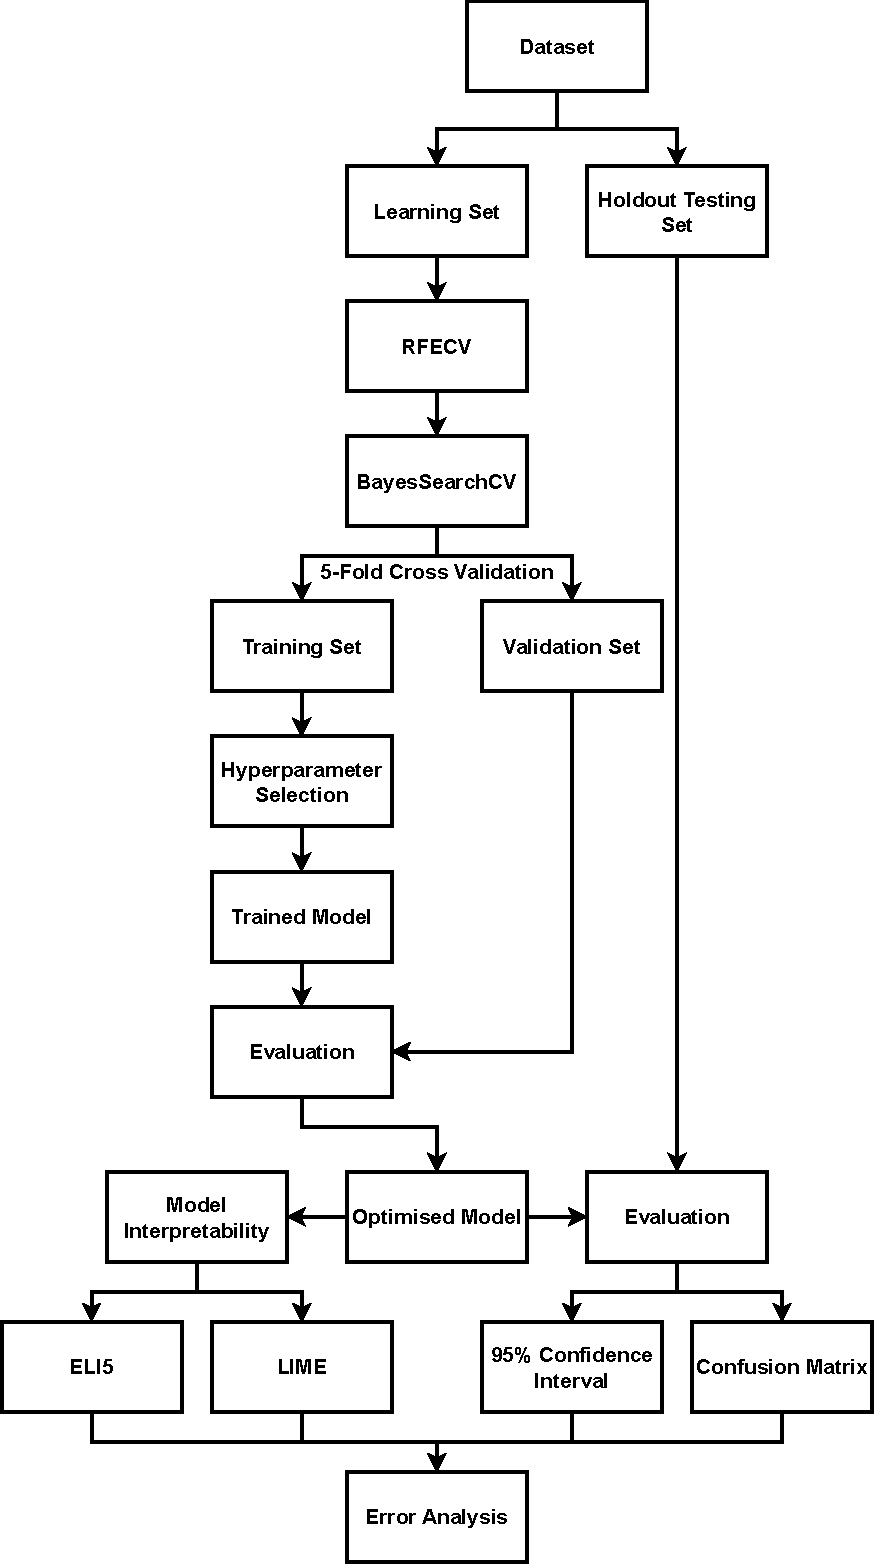
\includegraphics[width=0.83\linewidth]{images/Model_Training.pdf}    
    \caption{Figure showcasing our model training process.}
    \label{fig:Model_Training} 
\end{figure}

\begin{figure*}[!h]
    \centering
    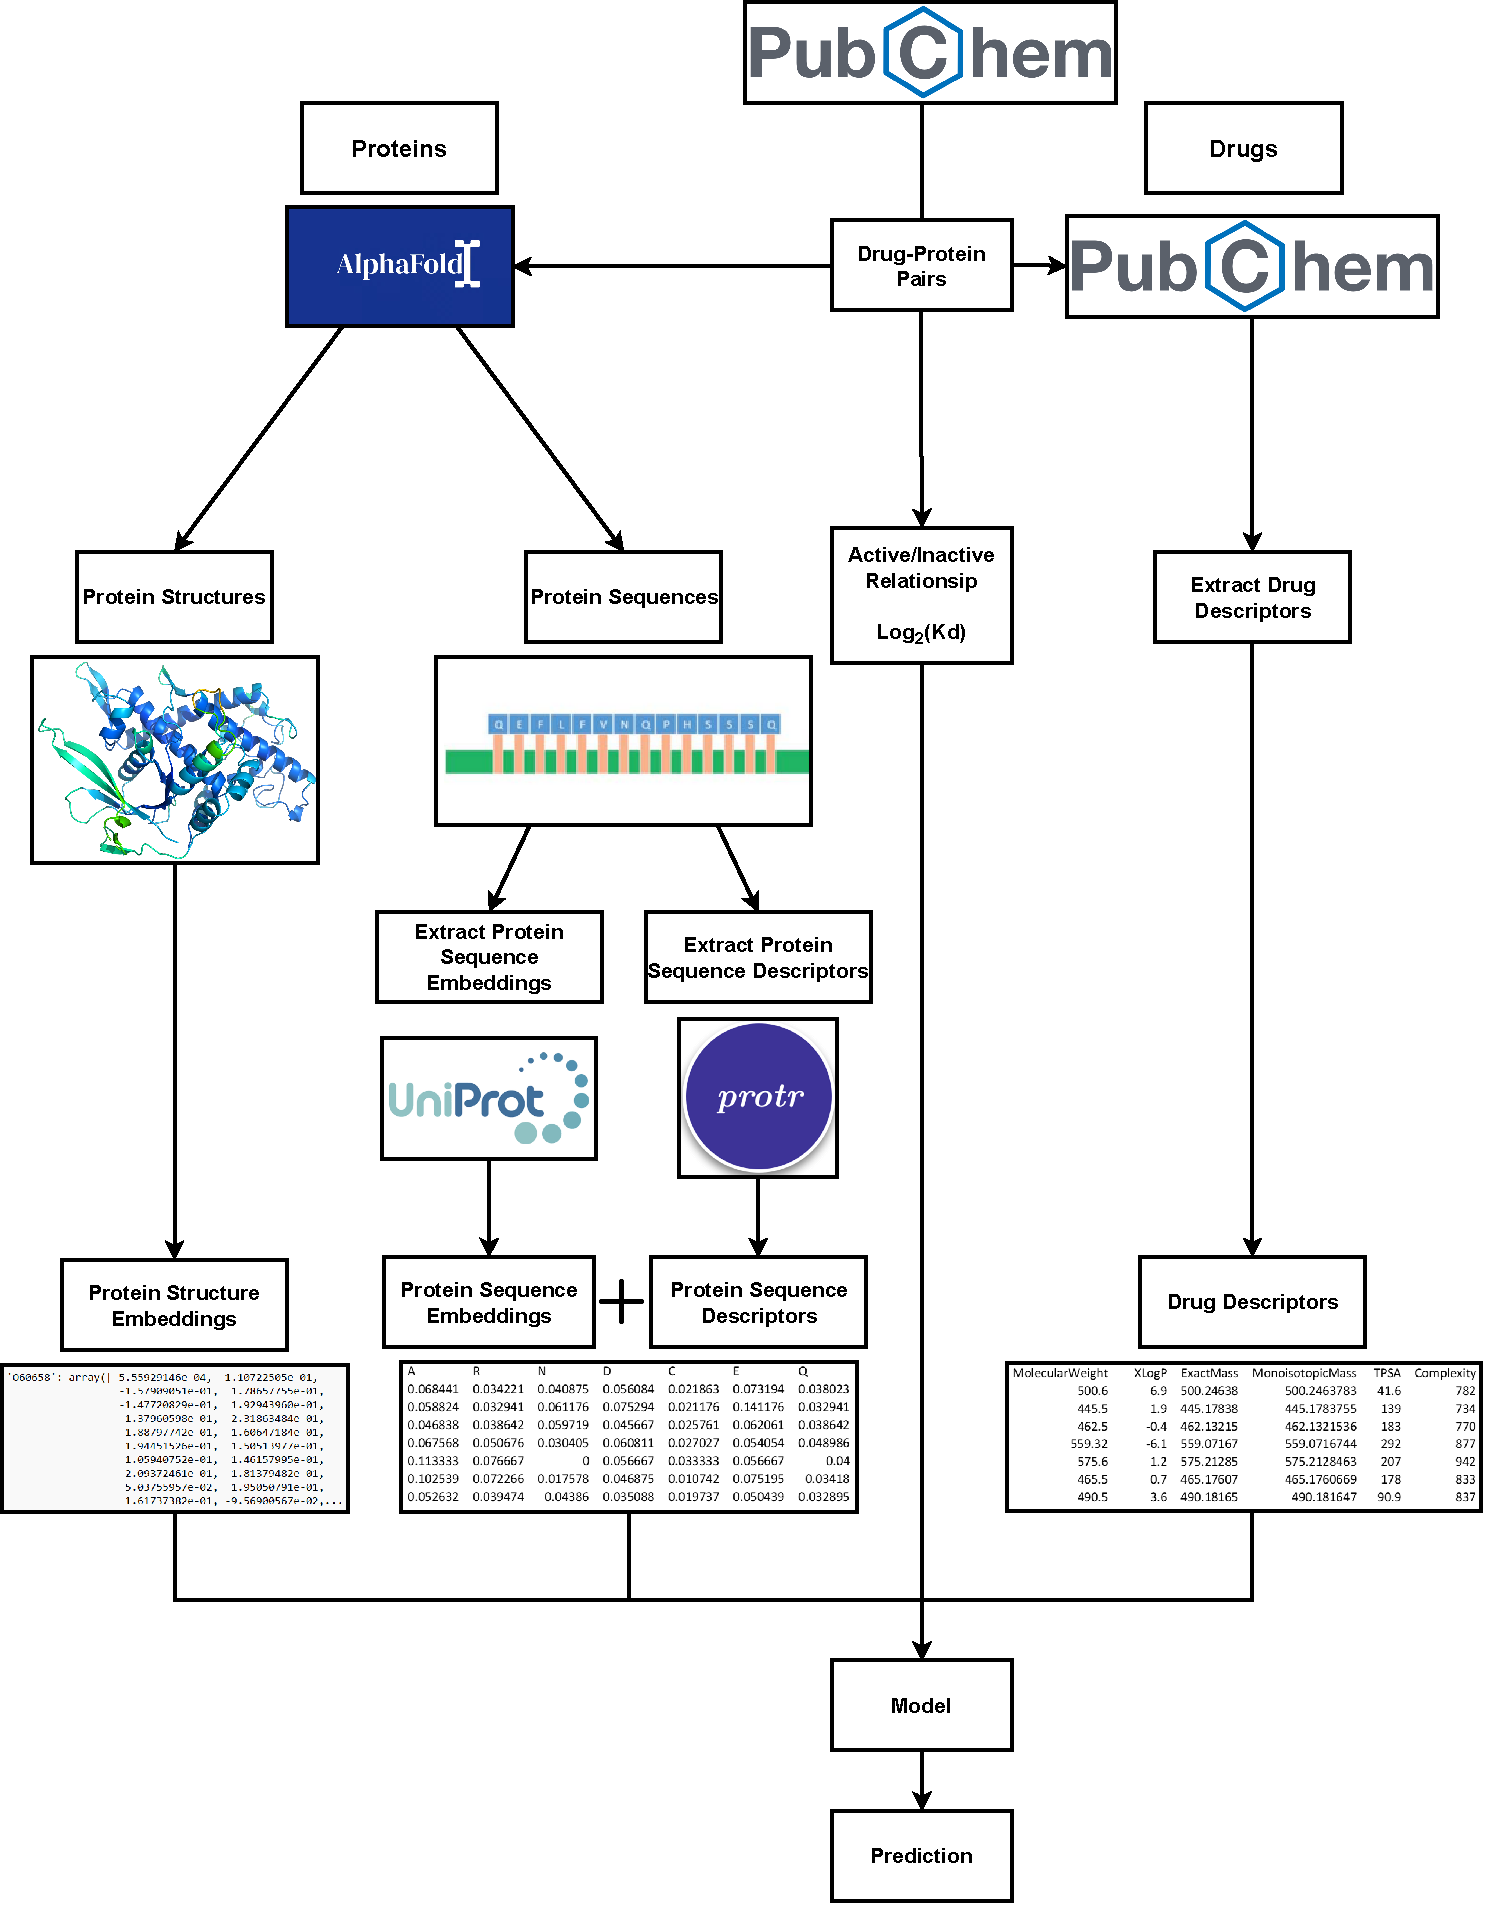
\includegraphics[width=0.95\linewidth]{images/DTIs_Methodology.pdf}    
    \caption{Figure showcasing our methodology behind the DTI models.}
    \label{fig:DTIs_Methodology} 
\end{figure*}